\documentclass[fleqn,aspectratio=169,10pt]{beamer}
\usetheme{Madrid}
\usepackage[T1]{fontenc}
\begingroup
\catcode`_=\active
\gdef\literalunderscores #1{%
    \catcode`_=\active
    \def_{\_}%
    \scantokens{#1}%
}
\endgroup

\newcommand*{\cmd}[1]{\pmb{\mathrm{\protect\literalunderscores{#1}}}}
\newcommand*{\tvar}[1]{\mathrm{\mathit{\textrm{\textquotesingle}#1}}}
\newcommand*{\singlequote}{\textrm{\textquotesingle}}
\newcommand*{\type}[1]{\mathrm{\mathit{#1}}}
\newcommand*{\const}[1]{\mathrm{\mathsf{\protect\literalunderscores{#1}}}}
\newcommand*{\specon}[1]{\literalunderscores{#1}}
\newcommand*{\var}[1]{\mathrm{\mathit{#1}}}
\newcommand*{\syntax}[1]{\mathrm{\mathsf{\underline{#1}}}}
\newcommand*{\literal}[1]{\mathrm{\texttt{#1}}}

\newlength\isawidth
\newcommand*{\isabelleinner}{%
    \let\isaoldnewline=\\%
    \renewcommand{\\}{\setlength\isawidth{\linewidth}\isaoldnewline}%
    \setlength\isawidth{\linewidth}%
    \relpenalty=700%
}
\newenvironment{isabelle}{\list{}{}\item[]\isabelleinner}{\endlist}
\newenvironment{isabelle*}{\begingroup\isabelleinner}{\endgroup}
\newcommand*{\isa}[1]{\parbox[t]{\isawidth}{%
        \raggedright%
        \renewcommand{\\}{\isaoldnewline}%
        \setlength\hangindent{1em}%
        \strut \!\begin{align*}\displaystyle #1\end{align*}%
}}
\newcommand{\isabelleinline}[1]{$#1$}

\newcommand{\more}{\hspace*{1em}\addtolength{\isawidth}{-1em}}
\newcommand{\bmore}{\leavevmode\rlap{\hspace{0.2em}$|$}\more}
\newcommand{\less}{\hspace*{-1em}\more}
\newcommand{\bless}{\hspace*{-1em}\bmore}

\let\phi=\varphi
\newcommand{\oftype}{\mathrel{::}}
\newcommand{\Fun}{\Rightarrow}
\newcommand*{\PartialFun}{\rightharpoonup}
\newcommand{\Interval}{\mathcal{I}}
\newcommand{\Implies}{\longrightarrow}
\newcommand{\Forall}{\forall}
\newcommand{\Exists}{\exists}
\newcommand{\Andd}{\wedge}
%% \newcommand{\Or}{\lor}
\newcommand{\Iff}{\longleftrightarrow}

\mathcode`\#="2023
\mathcode`@="2040
\mathcode`!="2021
\newcommand{\Nil}{[\,]}
\newcommand{\Image}{\mathbin{\specon{\grave{}}}}
\newcommand{\InvImage}{\mathbin{{\text -}\const{\grave{}}}}
\newcommand{\MapThe}[1]{\overline{#1}}
\newcommand{\Upt}{\mathrel{..\mathrm{<}}}
\newcommand{\GreaterThanAtMost}{\mathrel{\mathrm{<}..}}
\newcommand{\None}{\bot}
\newcommand*{\Some}[1]{\langle #1\rangle}
\newcommand*{\Union}{\cup}
\newcommand*{\Intersection}{\cap}
\newcommand*{\Emptyset}{\{\}}

\newcommand{\Imp}{\rightarrow}
\newcommand{\Prev}{\operatorname{\CIRCLE}}
\newcommand{\Next}{\operatorname{\Circle}}
\newcommand{\Since}{\mathbin{\mathsf{S}}}
\newcommand{\Until}{\mathbin{\mathsf{U}}}
\newcommand{\Always}{\operatorname{\square}}
\newcommand{\PAlways}{\operatorname{\blacksquare}}
\newcommand{\Eventually}{\operatorname{\lozenge}}
\newcommand{\Once}{\operatorname{\blacklozenge}}

\newcommand{\SRel}{\const{Eq}_{\const{S}}}
\newcommand{\SPred}{\const{Pred}_{\const{S}}}
\newcommand{\SExists}{\const{Exists}_{\const{S}}}
\newcommand{\SAnd}{\const{And}_{\const{S}}}
\newcommand{\SOr}{\const{Or}_{\const{S}}}
\newcommand{\SNext}{\const{Next}_{\const{S}}}
\newcommand{\SPrev}{\const{Prev}_{\const{S}}}
\newcommand{\SSince}{\const{Since}_{\const{S}}}
\newcommand{\SUntil}{\const{Until}_{\const{S}}}

\newcommand{\Exfrm}{\phi_{\mathit{ex}}}
\newcommand{\Exprefix}{\pi_{\mathit{ex}}}

\newcommand*{\Univ}{\mathfrak{U}}

\newcommand*{\BulkBenq}[2]{{#1} \gg {#2}}

\newcommand*{\assoc}{\curvearrowleft}
\newcommand*{\reassoc}{\curvearrowright}

\newcommand*{\IdOp}{\mathcal{I}}
\newcommand*{\TranspOp}{\mathcal{X}}
\newcommand*{\Scomp}[2]{{#1} \bullet {#2}}
\newcommand*{\Pcomp}[2]{{#1} \parallel {#2}}
\newcommand*{\Feedback}[1]{{#1} \uparrow}
\newcommand*{\EndOp}{\oslash}
\newcommand*{\SilentOp}{\odot}
\newcommand*{\SpinOp}{\otimes}
\newcommand*{\SourceOp}{\rotatebox[origin=c]{180}{!}}
\newcommand*{\SinkOp}{!}
\newcommand*{\MergeOp}{\mathcal{V}}
\newcommand*{\SplitOp}{\Lambda}
\newcommand*{\AeqOp}{\mathcal{Q}}
\newcommand*{\AcopyOp}{\mathcal{C}}
\newcommand*{\PreBuf}{\dashv}
\newcommand*{\PostBuf}{\vdash}

\newcommand*{\bisim}[2]{{#1} \sim {#2}}
\newcommand*{\wbisim}[2]{{#1} \approx {#2}}
\newcommand*{\TraceEquiv}[2]{{#1} \equiv_t {#2}}

\newcommand*\highlight[1]{\mbox{\setlength{\fboxsep}{0pt}\colorbox{gray!30}{\strut$#1$}}}

\newcommand*{\circled}[1]{\tikz[baseline=(char.base)]{
  \node[shape=circle,draw,inner sep=0] (char) {#1};}}
\newcommand*{\ogt}{\circled{>}}
\newcommand*{\olt}{\circled{<}}


\usepackage{wasysym}
\usepackage{fancybox,graphicx,hyperref,url}
\usepackage{tikz}
\usetikzlibrary{shapes,arrows}
\usetikzlibrary{positioning}
\usepackage{booktabs}
\usepackage{enumitem}

\usepackage{listings}
\usepackage{pdfpages}
\usepackage{lstautogobble}

\usepackage[listings,skins,breakable,xparse,most]{tcolorbox}
\tcbuselibrary{theorems}
\tcbset{highlight math/.append style={boxrule=0pt,
                                      frame hidden,
                                      colback=yellow!40!white,
                                      sharp corners}}

\usepackage{xpatch}

\usepackage{realboxes}
\usetikzlibrary{fit}
\usetikzlibrary{shadings}
\usetikzlibrary{shapes.arrows,shadows.blur}

\pgfdeclarefunctionalshading{Hermite-Gaussian modes}{\pgfpoint{-25bp}{-25bp}}{\pgfpoint{25bp}{25bp}}{}{
    10 atan sin 1000 mul cos 1 add
    exch
    10 atan sin 1000 mul cos 1 add
    mul 4 div
    dup dup
}

\makeatletter
\xpretocmd\lstinline{\Colorbox{yellow!10!white}\bgroup\appto\lst@DeInit{\egroup}}{}{}
\makeatother

\definecolor{my_red}{RGB}{128, 0, 0}

\lstset{captionpos=b}
\lstset{numberbychapter=false}
\lstset{autogobble}
% \lstset{breaklines=true}

\usepackage{tikz}
\usepackage{subcaption}
\usetikzlibrary{calc, chains, decorations.pathmorphing}
\usetikzlibrary{shapes,arrows,backgrounds}
\usetikzlibrary{positioning,fit,shapes.geometric,shapes}

\setbeamercovered{transparent}

\setlistdepth{9}
\setlist[itemize,1]{label=$\bullet$}
\setlist[itemize,2]{label=$\bullet$}
\setlist[itemize,3]{label=$\bullet$}
\setlist[itemize,4]{label=$\bullet$}
\setlist[itemize,5]{label=$\bullet$}
\setlist[itemize,6]{label=$\bullet$}
\setlist[itemize,7]{label=$\bullet$}
\setlist[itemize,8]{label=$\bullet$}
\setlist[itemize,9]{label=$\bullet$}
\renewlist{itemize}{itemize}{9}

\setlist[enumerate,1]{label=$\arabic*.$}
\setlist[enumerate,2]{label=$\alph*.$}
\setlist[enumerate,3]{label=$\roman*.$}
\setlist[enumerate,4]{label=$\arabic*.$}
\setlist[enumerate,5]{label=$\alpha*$}
\setlist[enumerate,6]{label=$\roman*.$}
\setlist[enumerate,7]{label=$\arabic*.$}
\setlist[enumerate,8]{label=$\alph*.$}
\setlist[enumerate,9]{label=$\roman*.$}
\renewlist{enumerate}{enumerate}{9}

\AtBeginSection[]{
  \begin{frame}[noframenumbering]
    \vfill
    \centering
    \begin{beamercolorbox}[sep=8pt,center,shadow=true,rounded=true]{title}
      \usebeamerfont{title}\insertsectionhead\par%
    \end{beamercolorbox}
    \vfill
  \end{frame}
}

\title[Nondeterministic Asynchronous Dataflow in Isabelle/HOL]{Nondeterministic Asynchronous Dataflow in Isabelle/HOL}

\author[Rafael, Laouen and Dmitriy]{
  \underline{Rafael Castro G. Silva}, Laouen Fernet and  Dmitriy Traytel\\\medskip
  }
% {\small \url{rasi@di.ku.dk}}

\date{14/05/2025}

% change title (done)
% (co)datatypes -> codatatypes (done)
% while_option from HOL library (done)
% coindtive principle -> coinduction principle (done)
% remove next step slide, andd as a bullet (done)
% explain slice in more detail (done)
% mention selectors in llist slide, drop lmap, drop lset (done)
% move count operator example to slide that introduce op type (done)
% modeling lazy list processors which do not care about time (done)
% reduce Corecursion is like recursion line (done)
% why partial order? mention timely dataflow (done)
% explain what incremental, and set expectation for example (done)
% move arrows (done)
% Change push to out, done to out (done)
% put star footnote on op type saying it is simplified compare to the paper, also in the composition lemma (done)
% write the lapp lemma about lfinite (done)
% show coinduction principle for llist (done)
% add link llist afp (done)
% on produce slide, metion lshift as friend (point to freinds with benefits paper) (done)
% justify the compositional reasoning with lines of code for each building block (done)
% slide about tecnicques used, coinduction principles, friends, reasoning up to friends, generalization using skip_op, combining coinduction and induction, coinduction up to congruence for coinductive predicates, say our paper is more detailed in these topics
%
% add definition of batch_op, and all 4 properties

\institute[UCPH]{
  Department of Computer Science \\
  University of Copenhagen}

\begin{document}
\setbeamercovered{invisible}
% \setbeamercovered{dynamic}

\begin{frame}
  \titlepage
\end{frame}

\section{Motivation}

\begin{frame}[fragile]
  \frametitle{Motivation}
  \begin{block}{Context:}
  \begin{itemize}
    \item Stream Processing: programs that compute (possibly) unbounded sequences of data (streams)
    \item A common problem in the industry
    \item Frameworks: Apache Flink, Google Cloud Dataflow, and Timely Dataflow
          \begin{figure}
            \centering
            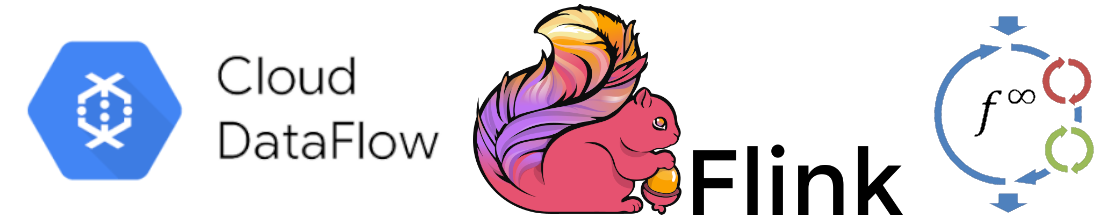
\includegraphics[scale=0.1]{all}
          \end{figure}
    \item Why use frameworks?
          \begin{itemize}
            \item Highly Parallel
            \item Low latency (output as soon as possible)
            \item Incremental computing (re-uses previous computations)
          \end{itemize}
  \end{itemize}
  \pause
  \end{block}
  \begin{block}{Our goal:}
    Mechanically Verify Timely Dataflow algorithms
  \end{block}
\end{frame}

\section{A Good Foundation}

\begin{frame}[fragile]
  \frametitle{A Good Foundation}
  \begin{columns}
    \begin{column}{.35\textwidth}
      \begin{figure}
        \centering
        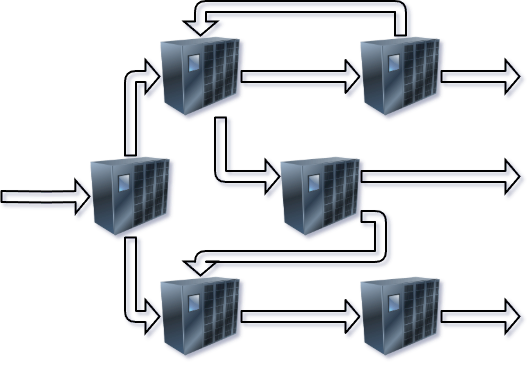
\includegraphics[width=1\textwidth]{network.png}
      \end{figure}
    \end{column}
    \begin{column}{.65\textwidth}
      \begin{itemize}
        \item Nondeterministic Asynchronous Dataflow
              \begin{itemize}
                \pause
                \item Dataflow: Directed graph of interconnected operators
                \pause
                \item Asynchronous:
                      \begin{itemize}
                        \item Operators execute independently:\\ processes without an orchestrator
                        \item Operators can freely communicate with the network (read/write); do silent computation steps
                        \item Networks are unbounded FIFO queues
                      \end{itemize}
                \pause
                \item Nondeterministic:
                      \begin{itemize}
                        \item Operators can make nondeterministic choices
                      \end{itemize}
              \end{itemize}
      \end{itemize}
    \end{column}
  \end{columns}
\end{frame}

\begin{frame}[fragile]
  \frametitle{The Algebra for Nondeterministic Asynchronous Dataflow}
  \begin{columns}
    \begin{column}{.6\textwidth}
      \begin{itemize}
        \item Bergstra et al. presents an algebra for Nondeterministic Asynchronous Dataflow
        \item Primitives:\\
              sequential and parallel composition; feedback loop...
        \item 52 axioms
        \item A process calculus instance
      \end{itemize}
    \end{column}
    \begin{column}{.4\textwidth}
      \begin{figure}
        \centering
        \shadowbox{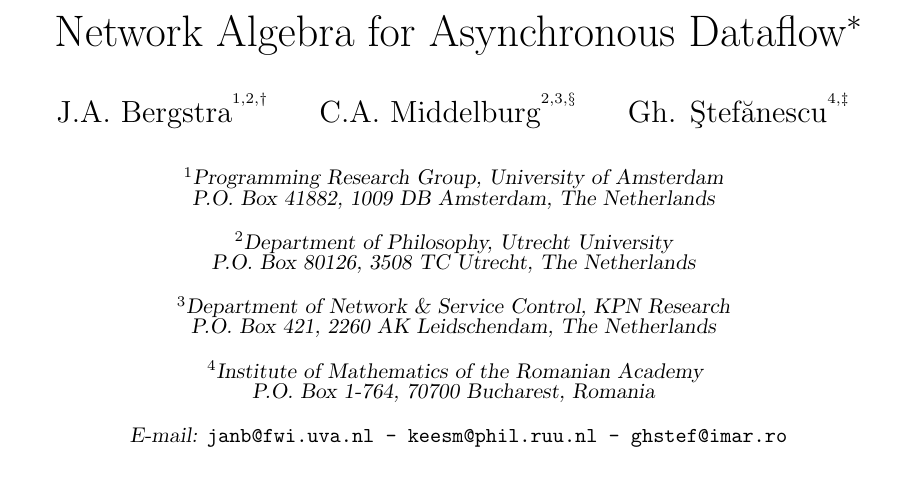
\includegraphics[width=0.9\textwidth]{Bergstra.png}}
      \end{figure}
    \end{column}
  \end{columns}
\end{frame}

\begin{frame}[fragile]
  \frametitle{Main Contributions}
  \begin{itemize}
    \item A Isabelle/HOL instance of Nondeterministic Asynchronous Dataflow
          \begin{itemize}
            \item Operators as a shallow embedding as codatatypes
            \item 51 axioms proved
          \end{itemize}
    \item Executable via code extraction to Haskell
  \end{itemize}
\end{frame}

\section{Isabelle/HOL Preliminaries}

\begin{frame}[fragile]
  \frametitle{Isabelle/HOL}
  \begin{itemize}
    \item Classical higher-order logic (HOL):\\ Simple Typed Lambda Calculus + axiom of choice + axiom of infinity + rank-1 polymorphism
          \pause
    \item Isabelle: A generic proof assistant
          \begin{overlayarea}{\textwidth}{.3\textheight}
            \centering
            \begin{figure}
              \centering
              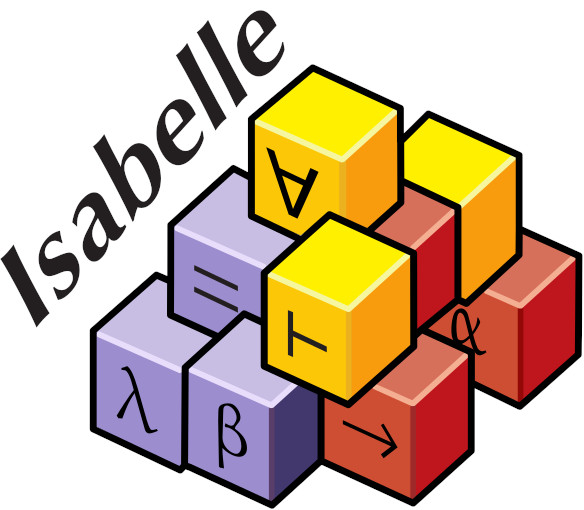
\includegraphics[scale=0.15]{isabelle}
            \end{figure}
          \end{overlayarea}
    \item Isabelle/HOL: Isabelle's flavor of HOL
  \end{itemize}
  \pause
    \begin{block}{Why Isabelle/HOL?}
      \begin{itemize}
        \item Codatatypes: (possibly) infinite data structures (e.g., lazy lists, streams)
        \item Corecursion: always eventually produces some codatatype constructor
        \item Coinductive predicate: infinite number of introduction rule applications
        \item Coinduction: reason about coinductive predicates
      \end{itemize}
  \end{block}

\end{frame}

\section{Operators as a Codatatype}

\begin{frame}[fragile]
  \frametitle{Operators}
  \vspace*{-2ex}
  \begin{tcolorbox}[enhanced,title=Operators in Isabelle/HOL,colback=yellow!30]
    \vspace*{-3ex}
    \hspace*{-5ex}
    \begin{align*}
      &   \cmd{codatatype}\ (\const{inputs}\!: \tvar{i}, \const{outputs}\!: \tvar{o}, \tvar{d})\ \type{op} =\\
      &   \more \const{Read}\ \tvar{i}\ (\tvar{d} \Fun (\tvar{i}, \tvar{o}, \tvar{d})\ \type{op})\ |\ \const{Write}\ ((\tvar{i}, \tvar{o}, \tvar{d})\ \type{op})\ \tvar{o}\ \tvar{d}\\
      &   \more \const{Silent}\ (\tvar{i}, \tvar{o}, \tvar{d})\ \type{op}\ |\ \const{Choice}\ ((\tvar{i}, \tvar{o}, \tvar{d})\ \type{op})\ \type{cset}
    \end{align*}
  \end{tcolorbox}

  \begin{columns}
    \begin{column}{.3\textwidth}
      \pause
      \begin{itemize}
        \item Type parameters: \\
              inputs/output ports; data
        \item Operator's actions
        \item inputs/outputs: \\
              Sets of used ports
        \item Possibly infinite trees
      \end{itemize}
    \end{column}
    \begin{column}{.22\textwidth}
      \pause
      \begin{tcolorbox}[enhanced,title=Uncommunicative operators,colback=yellow!30]
        \vspace*{-5ex}
        \hspace*{-8ex}
        \begin{tabular}{l l l}
          \hspace*{-4ex}
          \isa{
          & \more \EndOp = \const{Choice}\ \{\}_c
            }&
          \vspace*{-5ex}
          \\
          \hspace*{-4ex}
          \isa{
          & \more \SilentOp = \const{Silent}\ \SilentOp
            }&
          \vspace*{-5ex}
          \\
          \hspace*{-4ex}
          \isa{
          & \more \SpinOp = \const{Choice}\ \{\SpinOp\}_c
            }
        \end{tabular}
        \vspace*{-1ex}
      \end{tcolorbox}
    \end{column}
    \begin{column}{.48\textwidth}
      \pause
      \begin{tcolorbox}[enhanced,title=More examples,colback=yellow!30]
        \vspace*{-5ex}
        \hspace*{-8ex}
        \begin{tabular}{l l l}
          \hspace*{-2ex}
          \isa{
          \const{ex1} = \const{Choice}\ \{\const{Write}\ \const{ex1}\ 1\ 42, \EndOp\}_c
            }&
          \vspace*{-4ex}
          \\
          \hspace*{-2ex}
          \isa{
          \const{ex2} = \const{Choice}\ \{\const{Write}\ \const{ex2}\ 1\ 42, \const{ex2}\}_c
          }
          \vspace*{-4ex}
          \\
          \hspace*{-2ex}
          \isa{
          \const{ex3} = \const{Choice}\ \{\const{Write}\ \const{ex3}\ 1\ 42, \const{Silent}\ \const{ex3}\}_c
          }
        \end{tabular}
        \vspace*{-1ex}
      \end{tcolorbox}
    \end{column}
  \end{columns}
\end{frame}

\begin{frame}[fragile]
  \frametitle{Operators Equivalences: Motivation}
  \begin{block}{An ideal equivalence relation}
    \begin{itemize}
      \item Only equate operators that \textbf{behave} the same
      \item Useful reasoning principle
    \end{itemize}
  \end{block}
  \pause
  \begin{itemize}

          \begin{columns}
            \begin{column}{.42\textwidth}
              \item Milner's approach: Weak Bisimilarity
            \end{column}
            \begin{column}{.1\textwidth}
              \begin{figure}
                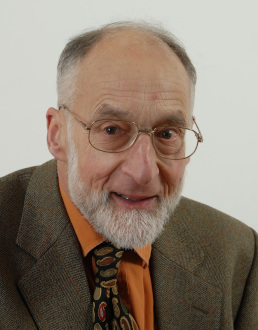
\includegraphics[width=1\textwidth]{milner.jpg}
              \end{figure}
            \end{column}
            \begin{column}{.1\textwidth}
                \includegraphics[width=1\textwidth]{book.jpg}
            \end{column}
            \begin{column}{.1\textwidth}
            \end{column}
          \end{columns}
          \item Based on labeled transition systems (LTS)
          \item Labels (actions): Read, Write, Silent ($\tau$)
  \end{itemize}
  % \begin{block}{Intuition}
  %   \footnotesize{Two operators are bisimilar if their corresponding transition systems can mutually simulate each other’s transitions.}
  % \end{block}
\end{frame}

\begin{frame}[fragile]
  \frametitle{Operators Equivalences: Label Transition System}
  \begin{tcolorbox}[enhanced,title=Label Transition System,colback=yellow!30]
    \vspace*{-3ex}
    \hspace*{-5ex}
    \begin{align*}
        &    \cmd{datatype}\ (\tvar{i}, \tvar{o}, \tvar{d})\ \type{IO} = \const{Inp}\ \tvar{i}\ \tvar{d}\ |\ \const{Out}\ \tvar{o}\ \tvar{d}\ |\ \const{Tau}
        \\[\jot]
        &    \cmd{inductive}\ \const{step}\ \cmd{where}\\
        &    \more \const{step}\ (\const{Inp}\ \var{p}\ \var{x})\ (\const{Read}\ \var{p}\ \var{f})\ (\var{f}\ \var{x}) \: \bmore \const{step}\ (\const{Out}\ \var{q}\ \var{x})\ (\const{Write}\ \var{op}\ \var{q}\ \var{x})\ \var{op} \\
        &    \bmore \const{step}\ \const{Tau}\ (\const{Silent}\ \var{op})\ \var{op} \\
        &    \bmore \var{op} \in_c \var{ops} \implies \const{step}\ \var{io}\ \var{op}\ \var{op}' \implies \const{step}\ \var{io}\ (\const{Choice}\ \var{ops})\ \var{op}'
    \end{align*}
  \end{tcolorbox}
\end{frame}

\begin{frame}[fragile]
  \frametitle{Operators Equivalences: Weak Bisimilarity}
    \vspace*{-2ex}
  \begin{tcolorbox}[enhanced,title=Weakly Simulates,colback=yellow!30]
    \vspace*{-4ex}
    \hspace*{-5ex}
    \begin{align*}
     & \const{estep}\ \const{Tau} = (\const{step}\ \const{Tau})^{==} \\
     & \const{estep}\ \var{io} = \const{step}\ \var{io}
    \\
    &  \const{wstep}\ \var{io} = (\const{step}\ \const{Tau})^{**}\ \const{OO}\ (\const{estep}\ \var{io})\ \const{OO}\ (\const{step}\ \const{Tau})^{**}
    \\
    & \const{wsim}\ \var{R}\ \var{op}_1\ \var{op}_2 = (\forall \var{io}\; \var{op}'_1.\ \const{step}\ \var{io}\ \var{op}_1\ \var{op}'_1 \Implies (\exists \var{op}'_2.\ \const{wstep}\ \var{io}\ \var{op}_2\ \var{op}'_2 \land \var{R}\ \var{op}'_1\ \var{op}'_2))
    \end{align*}
    \vspace*{-5ex}
  \end{tcolorbox}
  \vspace*{-1ex}
  \begin{itemize}
    \item A Relation \isabelleinline{\var{R}} is a \emph{weak simulation} if \isabelleinline{\forall \var{op}_1\; \var{op}_2.\ \var{R}\ \var{op}_1\ \var{op}_2 \Implies \const{wsim}\ \var{R}\ \var{op}_1\ \var{op}_2}.
  \end{itemize}
    \vspace*{-1.3ex}
  \pause
  \begin{tcolorbox}[enhanced,title=Weak Bisimilarity,colback=yellow!30]
    \vspace*{-3ex}
    \hspace*{-5ex}
    \begin{align*}
     & \cmd{coinductive}\ \const{wbisim}\ (\cmd{infix} \wbisim{}{} 40)\ \cmd{where}\\
     & \more \const{wsim}\ (\approx)\ \var{op}_1\ \var{op}_2 \implies \const{wsim}\ (\approx)\ \var{op}_2\ \var{op}_1 \implies \wbisim{\var{op}_1}{\var{op}_2}
    \end{align*}
    \vspace*{-5ex}
  \end{tcolorbox}
  \vspace*{-1ex}
  \begin{itemize}
    \item \isabelleinline{\var{R}} is a \emph{weak bisimulation} when both \isabelleinline{\var{R}} and its converse \isabelleinline{\var{R}^{\const{-1}}} are weak simulations. \\
          Weak bisimilarity is the largest weak bisimulation.
  \end{itemize}

  \pause
  \begin{itemize}
    \item $\approx$ has a useful coinduction principle
    \item $\EndOp \approx \SpinOp \approx \SilentOp$ and $\const{ex1} \approx \const{ex2} \approx \const{ex3}$
  \end{itemize}
\end{frame}

\section{Asynchronous Dataflow Operators}

\begin{frame}[fragile]
  \frametitle{Buffer Infrastructure}
  \begin{itemize}
    \item Buffers: $\tvar{a} \Fun \tvar{d}\ \type{list}$
  \end{itemize}
  \begin{tcolorbox}[enhanced,title=Auxiliary functions for buffers,colback=yellow!30]
    \vspace*{-3ex}
    \hspace*{-5ex}
    \begin{align*}
      & \const{BHD}\ \var{p}\ \var{buf} = \const{hd}\ (\var{buf}\ \var{p})
      \\
    & \const{BTL}\ \var{p}\ \var{buf} = \var{buf}(\var{p} := \const{tl}\ (\var{buf}\ \var{p}))
    \\
    & \const{BENQ}\ \var{p}\ \var{x}\ \var{buf} = \var{buf}(\var{p} := \var{buf}\ \var{p}\ \const{@}\ [\var{x}])
      \\
      & \BulkBenq{\var{buf}_1}{\var{buf}_2} = (\lambda \var{p}.\ \var{buf}_2\ \var{p}\ \const{@}\ \var{buf}_1\ \var{p})
    \end{align*}
  \end{tcolorbox}
\end{frame}

\begin{frame}[fragile]
  \frametitle{Identity}
  \begin{tcolorbox}[enhanced,title=Identity operator,colback=yellow!30]
    \vspace*{-3ex}
    \hspace*{-5ex}
    \begin{align*}
      & \const{id_op}\ \var{buf} = \const{Choice}
      \\
      & \only<2->{(((\lambda \var{p}.\ \const{Read}\ \var{p}\ (\lambda \var{x}.\ \const{id_op}\ (\const{BENQ}\ \var{p}\ \var{x}\ \var{buf})))\ \Image_c \ \Univ_c)\ }
      \\
      &\Union_c
      \\
      &\only<3->{\phantom{(}((\lambda \var{p}.\ \const{Write}\ (\const{id_op}\ (\const{BTL}\ \var{p}\ \var{buf}))\ \var{p}\ (\const{BHD}\ \var{p}\ \var{buf}))\ \Image_c \ \{\var{p} \in_c \Univ_c \mid \var{buf}\ \var{p} \neq []\}))}
    \end{align*}
  \end{tcolorbox}

  \only<2->{
    \begin{itemize}
            \only<2->{\item $\Univ_c$ is the set of usable ports provide by its type}
            \only<4->{\item Stream delayer!}
    \end{itemize}
  }

  \only<5->{
  \begin{tcolorbox}[enhanced,title=Identity operator with an empty buffer,colback=yellow!30]
    \vspace*{-3ex}
    \hspace*{-5ex}
    \begin{align*}
      \IdOp = \const{id_op}\ (\lambda \_.\ [])
    \end{align*}
  \end{tcolorbox}
  }
\end{frame}

\begin{frame}[fragile]
  \frametitle{Composition}
  \begin{itemize}
    \item foo
  \end{itemize}
\end{frame}

\begin{frame}[fragile]
  \frametitle{Asynchronous Dataflow Operators}
  \begin{itemize}
    \item foo
  \end{itemize}
\end{frame}

\section{Asynchronous Dataflow Properties}
\begin{frame}[fragile]
  \frametitle{Basic network algebra properties}
  \begin{figure}
    \centering
    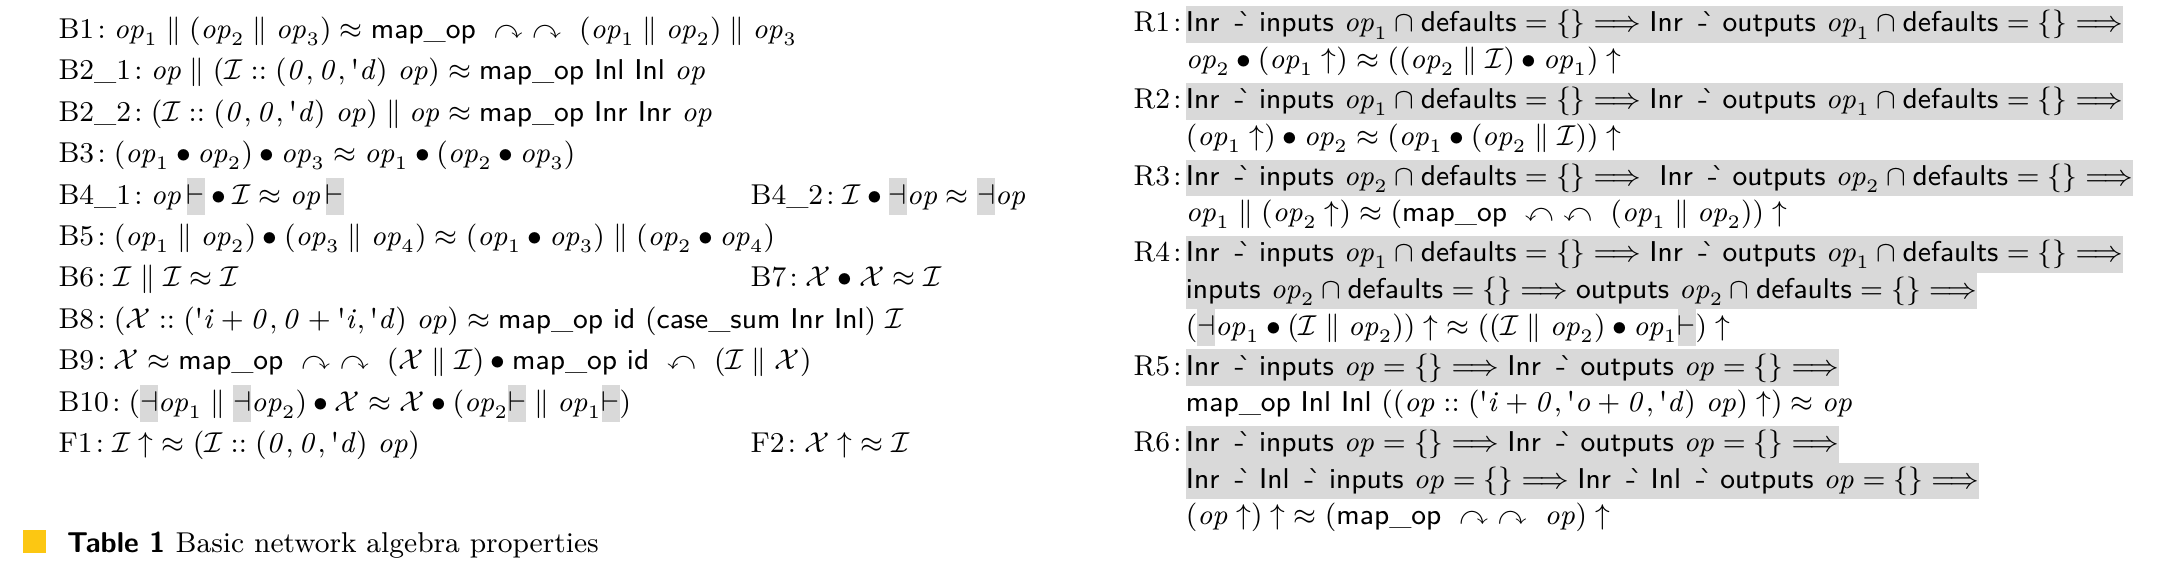
\includegraphics[width=1\textwidth]{table_1.png}
  \end{figure}
\end{frame}

\begin{frame}[fragile, noframenumbering]
  \frametitle{Basic network algebra properties}
  \begin{figure}
    \centering
    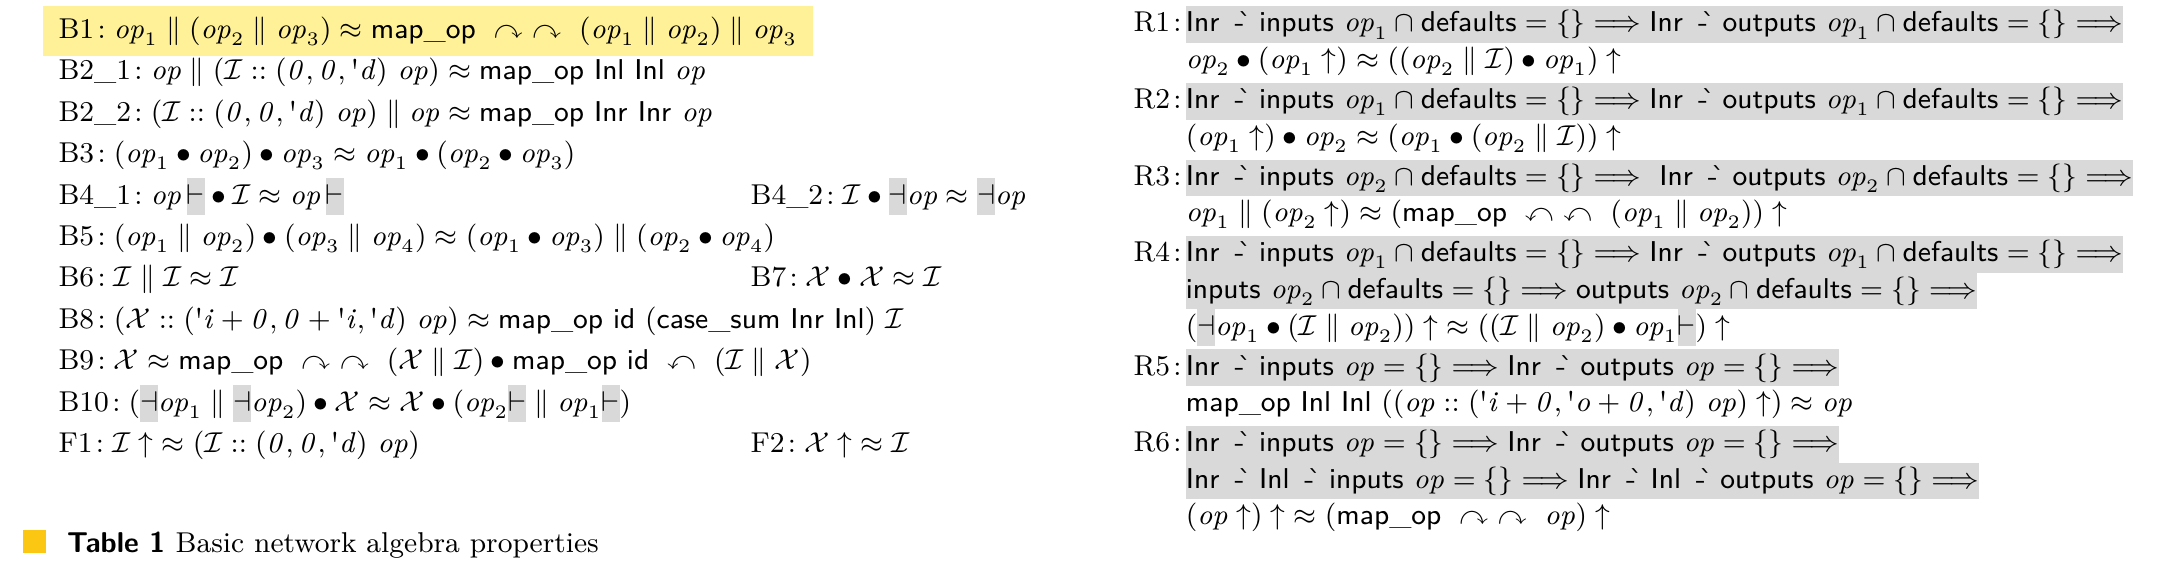
\includegraphics[width=1\textwidth]{table_1_1.png}
  \end{figure}
\end{frame}

\begin{frame}[fragile, noframenumbering]
  \frametitle{Basic network algebra properties}
  \begin{figure}
    \centering
    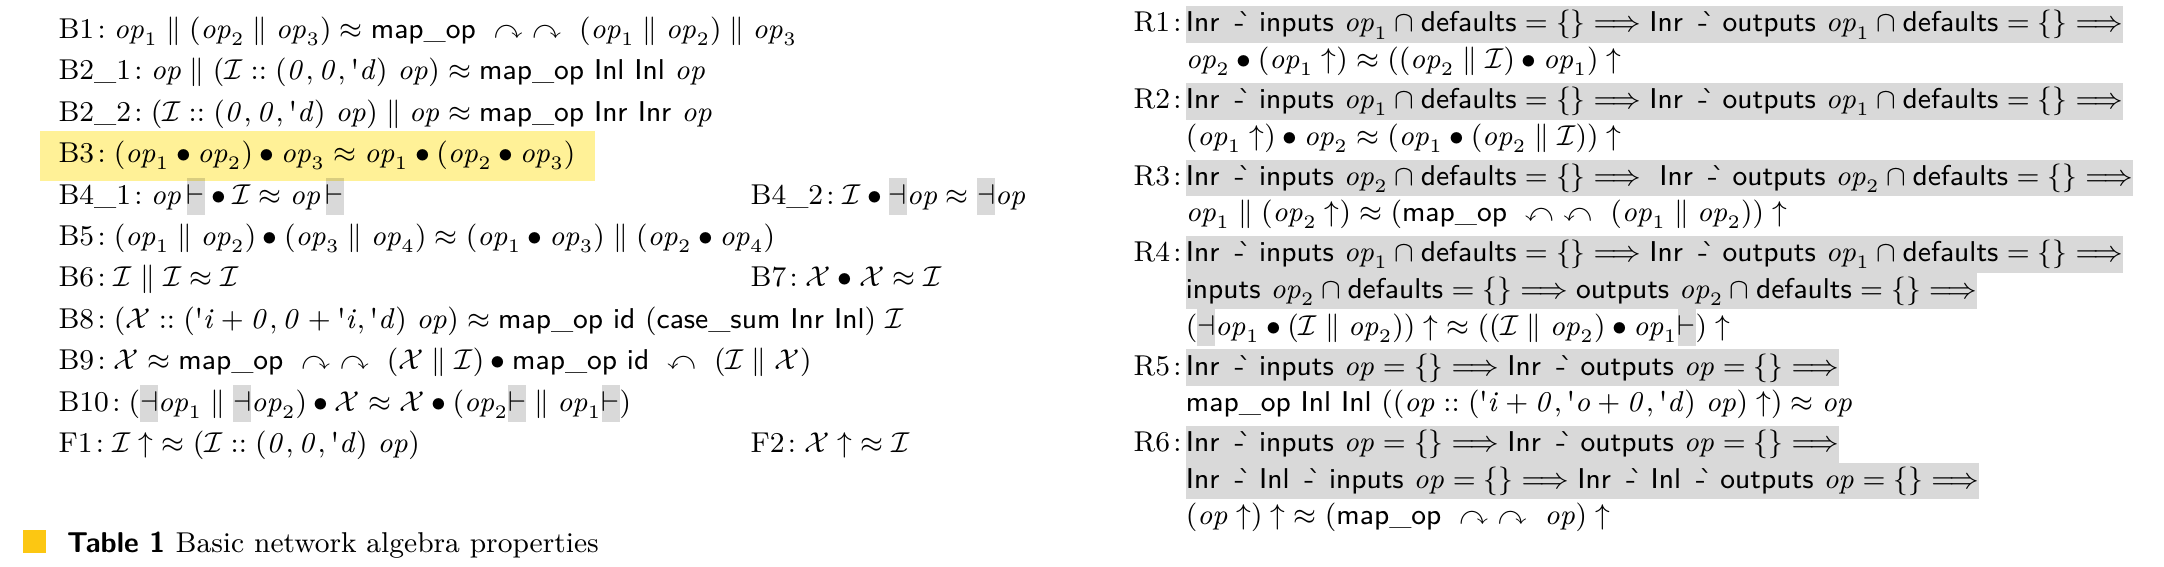
\includegraphics[width=1\textwidth]{table_1_2.png}
  \end{figure}
\end{frame}

\begin{frame}[fragile, noframenumbering]
  \frametitle{Basic network algebra properties}
  \begin{figure}
    \centering
    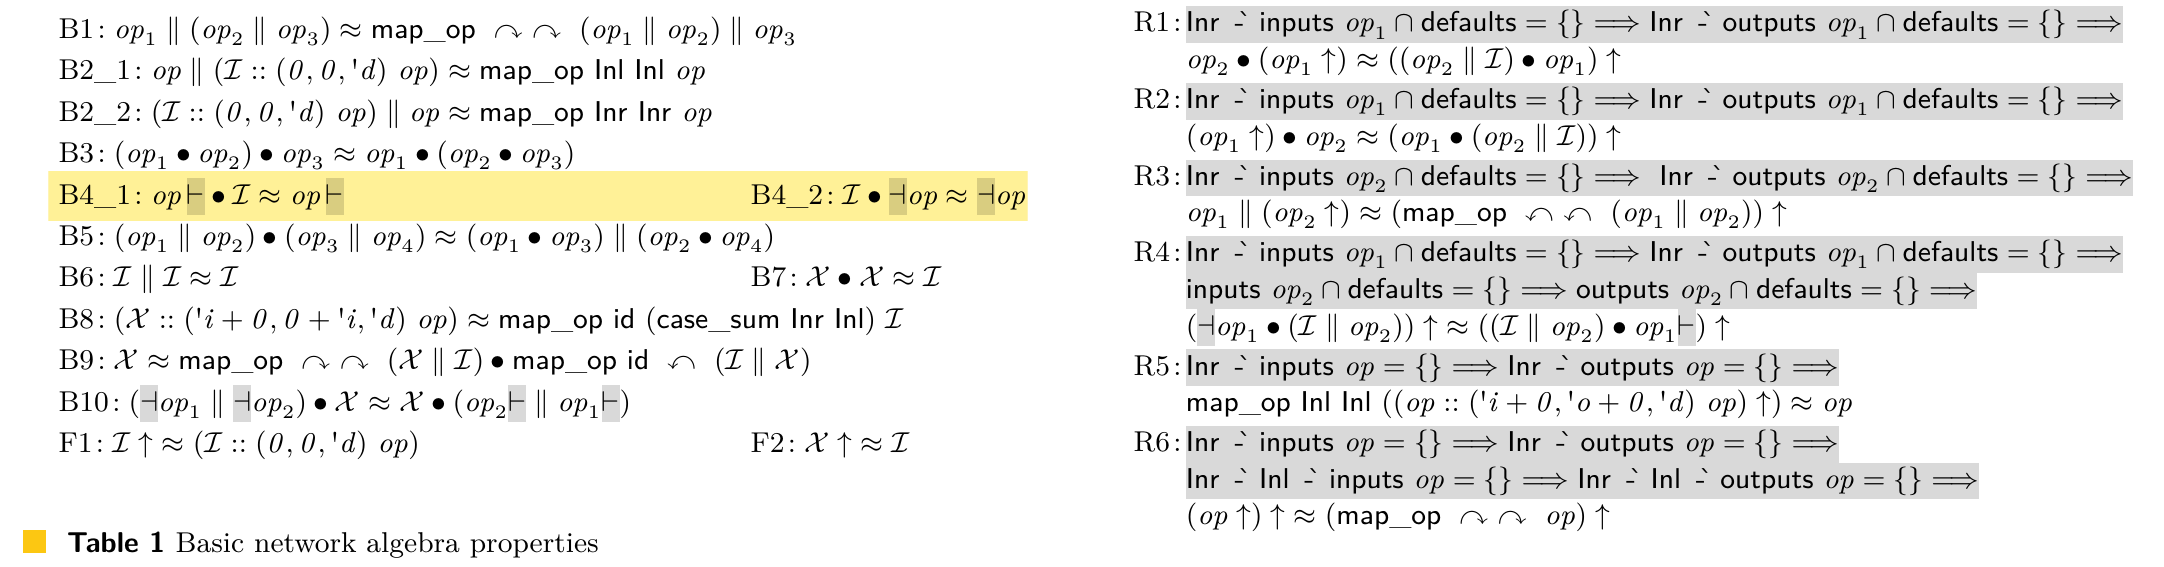
\includegraphics[width=1\textwidth]{table_1_3.png}
  \end{figure}
\end{frame}

\begin{frame}[fragile]
  \frametitle{Properties of equality test, merge, copy, split, source and sink operators}
  \begin{figure}
    \centering
    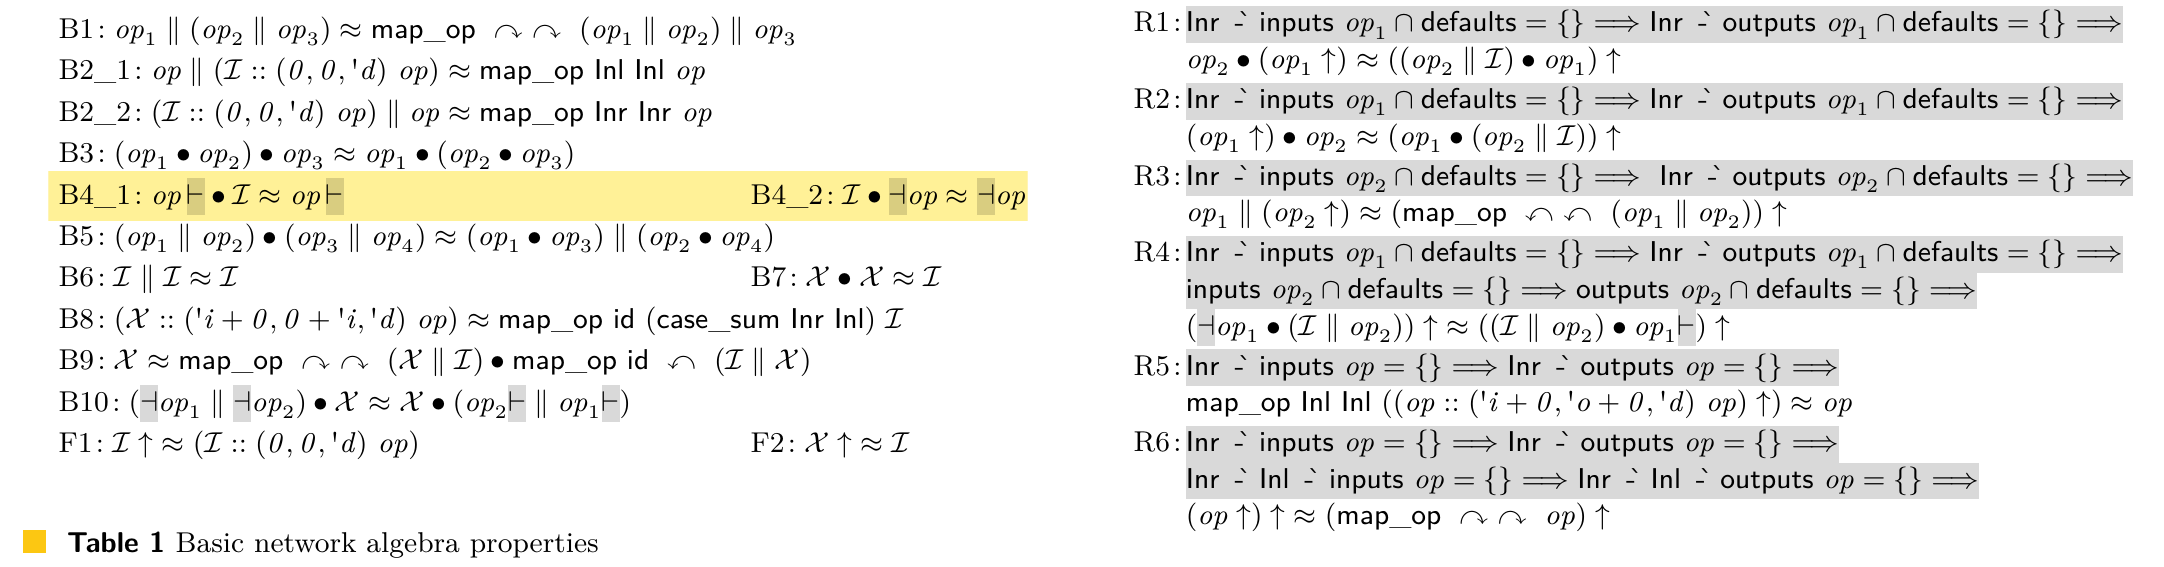
\includegraphics[width=1\textwidth]{table_1_3.png}
  \end{figure}
\end{frame}

\begin{frame}[fragile]
  \frametitle{A10}
  \begin{figure}
    \centering
    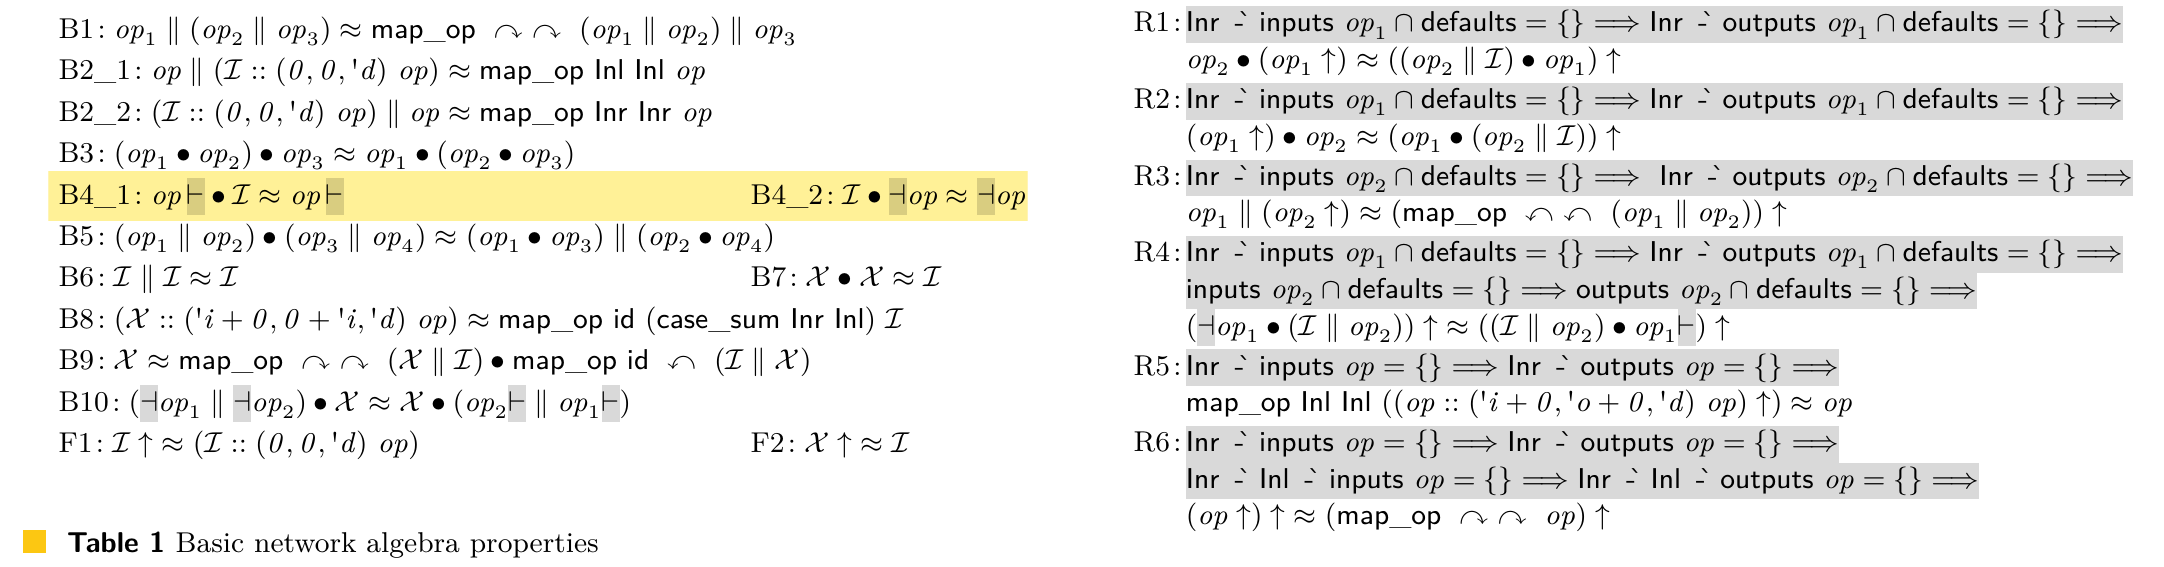
\includegraphics[width=1\textwidth]{table_1_3.png}
  \end{figure}
\end{frame}

\begin{frame}[fragile]
  \frametitle{Well-Behaved Operators}
  \begin{figure}
    \centering
    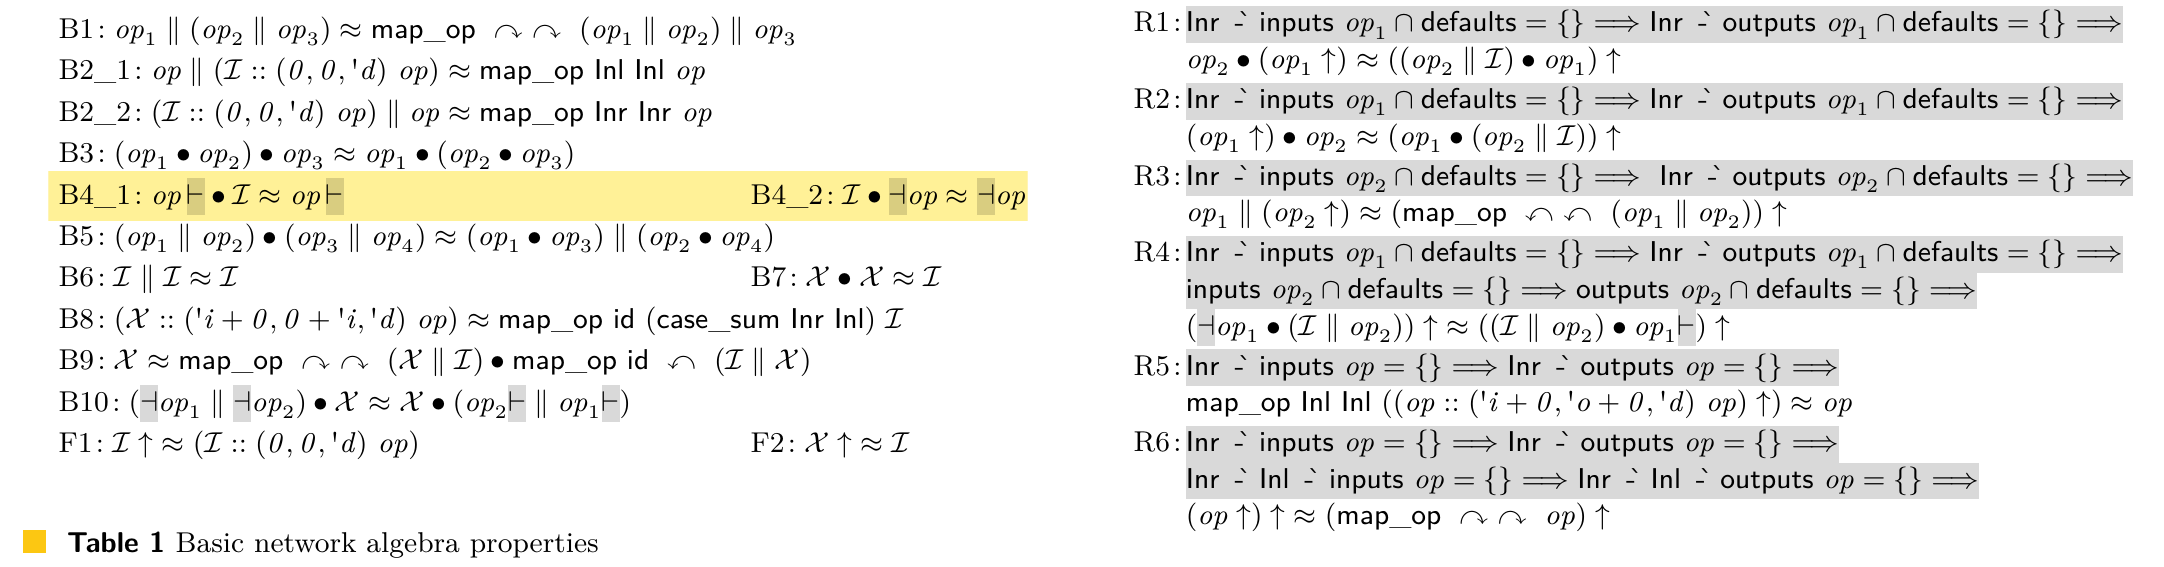
\includegraphics[width=1\textwidth]{table_1_3.png}
  \end{figure}
\end{frame}

\section{Related Work}

\begin{frame}[fragile]
  \frametitle{Related Work}
  \begin{itemize}
    \item A Isabelle/HOL instance of Nondeterministic Asynchronous Dataflow
          \begin{itemize}
            \item Operators as a shallow embedding as codatatypes
            \item 51 axioms proved
          \end{itemize}
    \item Executable via code extraction to Haskell
  \end{itemize}
\end{frame}

\section{Conclusion}
\begin{frame}
  \frametitle{Conclusion}
  \begin{itemize}
    \item Isabelle/HOL has a good tool set to formalize and reason about stream processing:
          \begin{itemize}
            \item Codatatypes, coinductive predicates, corecursion with friends, reasoning up to friends (congruence),
                  \begin{itemize}
                    \item Coinduction up to congruence principle is automatically derived for codatatypes (but not for coinductive principles)
                  \end{itemize}
          \end{itemize}
    \item Next step: Feedback loop
  \end{itemize}
\end{frame}
            %             slide about tecnicques used, coinduction principles, friends, reasoning up to friends, generalization using skip_op, combining coinduction and induction, coinduction up to congruence for coinductive predicates, say our paper is more detailed in these topics

\section{Questions, comments and suggestions}

\end{document}
